\documentclass{article}
\usepackage{tikz}
\usetikzlibrary{graphs,graphdrawing}
\usepackage{caption}
\usepackage[smartEllipses]{markdown}

\usepackage{multirow}
\usepackage{multicol}
\usepackage[framemethod=tikz]{mdframed}
\usepackage{lipsum}
\usepackage{tkz-graph}
\usegdlibrary{trees}
\usepackage{amsmath, amssymb}
\usepackage{pst-node}
\usepackage{blkarray}
\usepackage{amsmath, amssymb}
\usepackage{pst-node}

\usepackage[margin=2cm]{geometry}

\usepackage[utf8]{inputenc}
\begin{document}
	{Michele Beccari 856608 - Modelli Probabilistici per le decisioni -  Assignment 3 - Maggio 2023} 
	\section{Assignment 3}
Considerate il seguente gioco della “scalata”. Ci sono 5 livelli nel gioco, dove il livello 1 è il più basso (base) mentre il livello 5 è il più alto (cima). Un giocatore parte dalla base. Ad ogni iterazione viene lanciata una moneta non truccata. Se la moneta indica “testa” il giocatore sale di un livello. Se la moneta indica “croce” il giocatore si ritrova di nuovo alla base. 

Una volta arrivato alla cima il giocatore torna alla base se dal lancio della moneta esce “croce”, altrimenti rimane dove si trova (sempre in cima).

\begin{itemize}
	\item Trovare la matrice delle probabilità di transizione $P$.
\end{itemize}

\[
P = 
\begin{blockarray}{cccccc}
	& S_0 & S_1 & S_2 & S_3 & S_4 \\
	\begin{block}{c(ccccc)}
		S_0 &	0.5 &  0.5   & 0   & 0   & 0   \\
		S_1 &	0.5 &  0     & 0.5 & 0   & 0   \\
		S_2 &	0.5 &  0     & 0   & 0.5 & 0   \\
		S_3 &	0.5 &  0     & 0   & 0   & 0.5 \\
		S_4 &	0.5 &  0     & 0   & 0   & 0.5   \\
	\end{block}
\end{blockarray}
\]	

\begin{itemize}
	\item Trovare la matrice delle probabilità di transizione a due-step $P^2$	
\end{itemize}



\[
P^2 = 
\begin{blockarray}{cccccc}
	& S_0 & S_1 & S_2 & S_3 & S_4 \\
	\begin{block}{c(ccccc)}
		S_0 &	0.5 &  0.25   & 0.25 & 0     & 0      \\
		S_1 &	0.5 &  0.25   & 0    & 0.25  & 0      \\
		S_2 &	0.5 &  0.25   & 0    & 0     & 0.25   \\
		S_3 &	0.5 &  0.25   & 0    & 0     & 0.25    \\
		S_4 &	0.5 &  0.25   & 0    & 0     & 0.25   \\
	\end{block}
\end{blockarray}
\]	

\begin{itemize}
	\item Trovare la distribuzione stazionaria. 
\end{itemize}

\begin{mdframed}[hidealllines=true,backgroundcolor=blue!20]
	$P_{xy}$ indica la probabilità di arrivare allo stato $y$ partendo dallo stato $x$, indica quindi la entry $xy$-esima della matrice $P$
\end{mdframed} 

\begin{equation}
	\begin{cases}
		\pi_0 = P_{00} \cdot \pi_0 + P_{10} \cdot \pi_{1} + P_{20} \cdot \pi_2 + P_{30} \cdot \pi_3 +
		P_{40} \cdot \pi_4 \\
		
		\pi_1 = P_{01} \cdot \pi_0 + P_{11} \cdot \pi_{1} + P_{21} \cdot \pi_{2} + P_{31} \cdot \pi_3 +
		P_{41} \cdot \pi_4 \\
		
		\pi_2 = P_{02} \cdot \pi_0 + P_{12} \cdot \pi_{1} + P_{22} \cdot \pi_{2} + P_{32} \cdot \pi_3 +
		P_{42} \cdot \pi_4 \\
		
		\pi_3  = P_{03} \cdot \pi_0 + P_{13} \cdot \pi_{1} + P_{23} \cdot \pi_{2} + P_{33} \cdot \pi_3 +
		P_{43} \cdot \pi_4 \\
		
		\pi_4  = P_{04} \cdot \pi_0 + P_{14} \cdot \pi_{1} + P_{24} \cdot \pi_{2} + P_{34} \cdot \pi_3 +
		P_{44} \cdot \pi_4 \\
		
		1 = \pi_{0} + \pi_{1} + \pi_{2} + \pi_{3} + \pi_{4} 
	\end{cases}\
\end{equation}


Sostituendo con i valori noti otteniamo:
\begin{equation}
	\begin{cases}
		\pi_0 = 0.5 \cdot \pi_{0}  
		      + 0.5 \cdot \pi_{1} 
		      + 0.5 \cdot \pi_{2} 
		      + 0.5 \cdot \pi_{3} 
		      + 0.5 \cdot \pi_{4} \\
		
		\pi_1 = 0.5 \cdot \pi_{0}  
			  + 0   \cdot \pi_{1} 
			  + 0   \cdot \pi_{2} 
			  + 0   \cdot \pi_{3} 
			  + 0   \cdot \pi_{4} \\
		
		\pi_2 = 0    \cdot \pi_{0}  
		      + 0.5  \cdot \pi_{1} 
	          + 0   \cdot \pi_{2} 
		      + 0   \cdot \pi_{3} 
		      + 0   \cdot \pi_{4} \\
		      
		\pi_3 = 0    \cdot \pi_{0}  
		      + 0    \cdot \pi_{1} 
		      + 0.5   \cdot \pi_{2} 
		      + 0   \cdot \pi_{3} 
		      + 0   \cdot \pi_{4} \\      
		
		\pi_4 = 0    \cdot \pi_{0}  
              + 0    \cdot \pi_{1} 
              + 0    \cdot \pi_{2} 
              + 0.5  \cdot \pi_{3} 
              + 0.5  \cdot \pi_{4} \\  
		
		
		1 = \pi_{0} + \pi_{1} + \pi_{2} + \pi_{3} + \pi_{4} 
	\end{cases}\
\end{equation}
\begin{equation}
=	\begin{cases}
	\pi_0 = 0.5 \cdot \pi_{0}  
	+ 0.5 \cdot \pi_{1} 
	+ 0.5 \cdot \pi_{2} 
	+ 0.5 \cdot \pi_{3} 
	+ 0.5 \cdot \pi_{4} \\
	
	\pi_1 = 0.5 \cdot \pi_{0} \\
	
	\pi_2 = 0.5  \cdot \pi_{1}  \\
	
	\pi_3 =  0.5  \cdot \pi_{2}  \\      
	
	\pi_4 = 0.5   \cdot \pi_{3} + 0.5 \cdot \pi_{4}\\  
	
	
	1 = \pi_{0} + \pi_{1} + \pi_{2} + \pi_{3} + \pi_{4} 
\end{cases}\
\end{equation}


Notiamo che $\pi_{0} = 0.5 $ (lo deduciamo dalla prima e dall'ultima equazione del sistema):

\begin{equation}
	=	\begin{cases}
		\pi_0 = 0.5 \\
		
		\pi_1 = 0.5 \cdot \pi_{0} \\
		
		\pi_2 = 0.5  \cdot \pi_{1}  \\
		
		\pi_3 =  0.5  \cdot \pi_{2}  \\      
		
		\pi_4 = 0.5   \cdot \pi_{3} + 0.5 \cdot \pi_{4}\\  
		
		
		1 = \pi_{0} + \pi_{1} + \pi_{2} + \pi_{3} + \pi_{4} 
	\end{cases}\
\end{equation}

Da cui:

\[
	\pi_0 = 0.5 \\
\]
\[
	\pi_1 = 0.25 \\
\]
\[
    \pi_2 = 0.125 \\
\]
\[
    \pi_3 = 0.0625 \\
\]
\[
   \pi_4  = 0.0625 \cdot 0.5 + 0.5 \cdot \pi_4 \Longrightarrow  \pi_4 = 2 \cdot 0.0625 \cdot 0.5 =  0.0625  \\
\]

\pagebreak

\begin{center}
	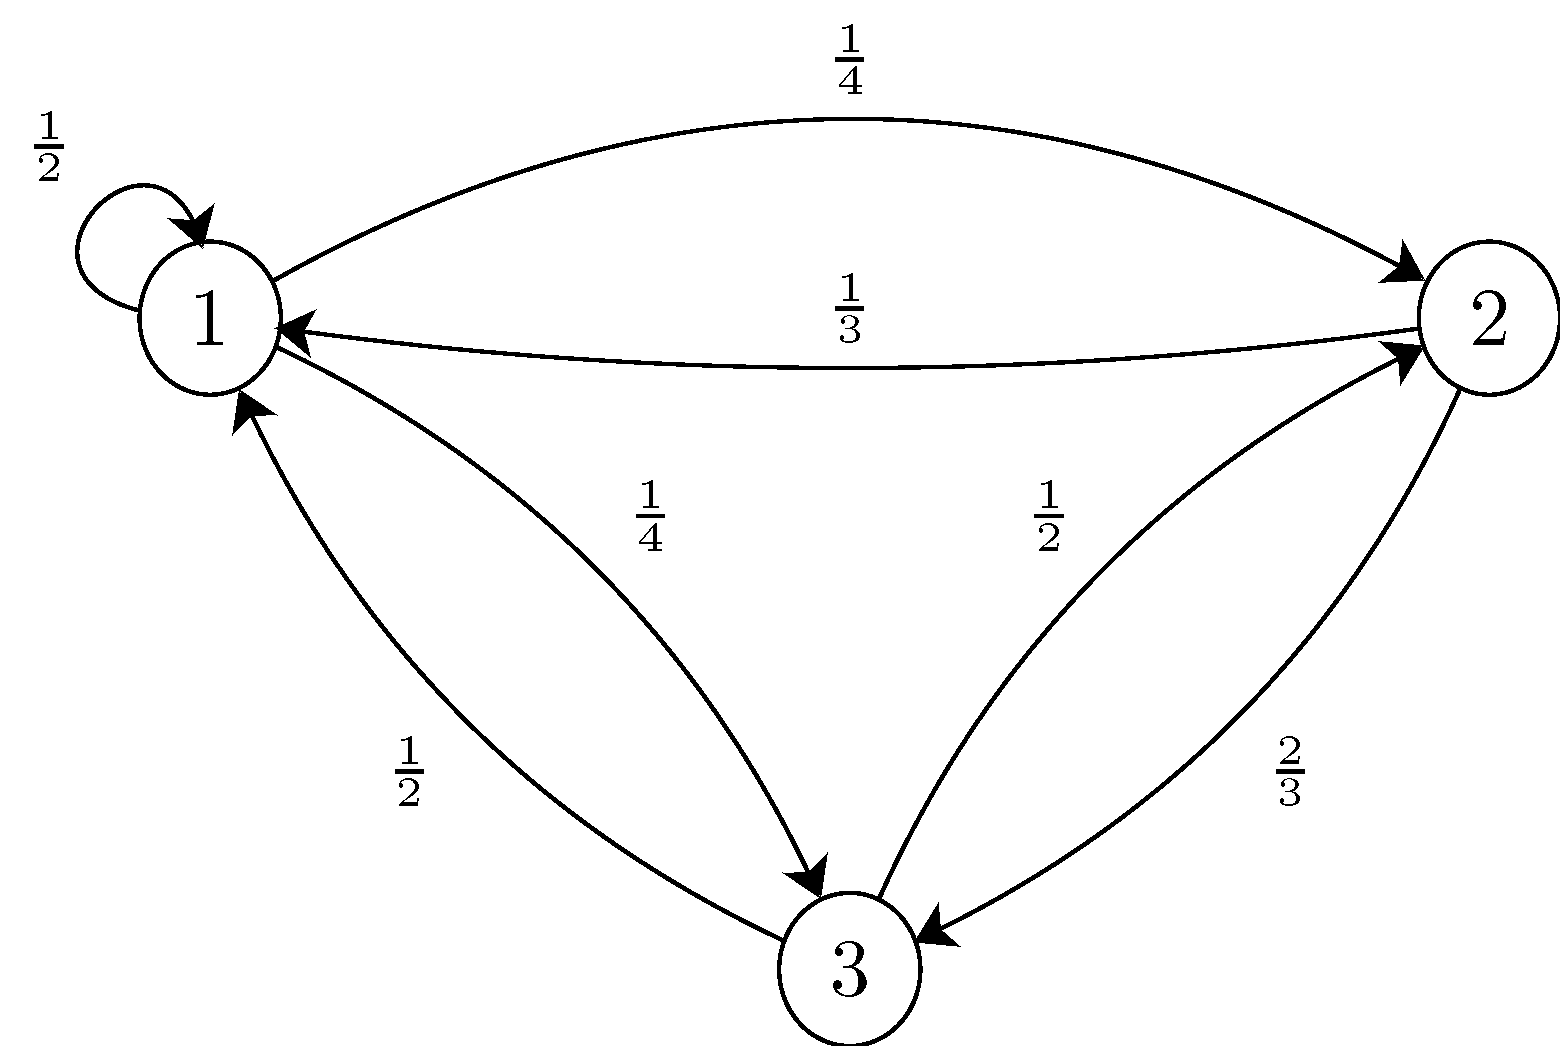
\includegraphics[width=10cm]{./immagini/mcmc.png}
\end{center}

\begin{itemize}
	\item Si consideri la catena di Markov  riportata in figura. La catena è irriducibile?
\end{itemize}

\begin{mdframed}[hidealllines=true,backgroundcolor=blue!20]
Una catena di Markov è detta irriducibile se tutti i suoi stati sono
comunicanti fra loro.
In altre parole, una catena di Markov è irriducibile se comunque dati due
vertici sul grafo ad essa associato esiste almeno un percorso orientato che li
collega.
\end{mdframed} 

In questo caso la catena di Markov è irriducibile:

\begin{itemize}
	\item 1 comunica direttamente sia con 2 che con 3 che con sè stesso
    \item 2 comunica direttamente con 3 e con 1, e comunicando con 1 (o con 2) comunica con sè stesso
    \item 3 comunica direttamente con 1 e con 2, e comunicando con 1 (o con 2) comunica con sè stesso
    
\end{itemize}


\begin{itemize}
	\item La catena è periodica? 
\end{itemize}

\begin{mdframed}[hidealllines=true,backgroundcolor=blue!20]
Uno stato i è periodico di periodo k>1 se k è il più piccolo
numero tale che tutti i cammini che dallo stato i ritornano ad i
hanno una lunghezza che è un multiplo di k.
\end{mdframed} 

La catena non è periodica: essendoci un cappio sul nodo 1 non è possibile trovare un numero $k > 1$ tale che tutti i cammini che dallo stato 1 tornino allo stato 1 in un numero di passi multiplo di $k$ (è possibile girare in loop un numero arbitrario di volte)




\pagebreak

\begin{itemize}
	\item Una catena di Markov irriducibile ammette sempre un’unica distribuzione di probabilità stazionaria.
\end{itemize}

Falso, la catena di Markov deve anche essere aperiodica

\begin{mdframed}[hidealllines=true,backgroundcolor=blue!20]
	Ogni catena di Markov aperiodica e irriducibile ha esattamente una distribuzione stazionaria.
\end{mdframed} 

Ad esempio la catena con questa distribuzione di probabilità $P$ non ammette distribuzione di probabilità stazionaria:

\[
P = 
\begin{blockarray}{ccc}
	& S_1 & S_2 \\
	\begin{block}{c(cc)}
		S_1  &  0     & 0.5 \\
		S_2  &  0.5   & 0 \\
	\end{block}
\end{blockarray}
\]


%Ad esempio la catena che segue non ha distribuzione stazionaria:
%
%\begin{markdown}
%      ┌──────────0.5─────────┐
%      │                      │
%      │                      │
%   ┌──▼───┐              ┌───┴───┐
%   │      │              │       │
%   │  1   │              │   2   │
%   │      │              │       │
%   └──┬───┘              └───▲───┘
%      │                      │
%      └───────────0.5────────┘ 
%\end{markdown}

\begin{flushleft}
	Una volta che un sistema entra in uno stato transiente in una catena di Markov, rimane in tale stato indefinitamente 
\end{flushleft}

Falso, lo stato transiente implica solo che esiste uno stato $j$ che è possibile raggiungere, ma non è possibile raggiungere lo stato corrente da j.

Non è detto che si rimanga in tale stato indefinitamente perchè sicuramente si può arrivare a j.

\end{document}



